\documentclass[a4paper,12pt]{ctexbeamer}
\usetheme{CambridgeUS}
\usepackage{amsmath}
\usepackage{amsfonts}
\usepackage{float}
\usepackage{enumerate}
\usepackage{svg}
\usepackage{graphicx}
\usepackage{booktabs}
\usepackage{ulem}
\usepackage{hyperref}
\title{保险法pre}
\author{董晨阳}
\date{\today}
\renewcommand{\indent}{\hspace*{2em}}
\begin{document}
\clearpage
\AtBeginSection[]
{
    \small\begin{frame}
        \frametitle{目录}
        \tableofcontents[
            sectionstyle=show/shaded,
            subsectionstyle=show/show/hide,
            subsubsectionstyle=show/show/show/hide
        ]
    \end{frame}
}
\maketitle

\section{保险资金运用管理办法(2018)}
\subsection{制定背景}
\begin{frame}
    \frametitle{法律背景}
    保险资金是指保险集团(控股)公司、保险公司以本外币计价的资本金、公积金、未分配利润、各项准备金以及其他资金。
    \begin{itemize}
        \item 2009年修订《保险法》:在银行存款、债券投资之外,增加不动产、股票及基金保险资金等运用形式
        \item 《保险资金运用管理暂行办法(2010)》:规定投资比例,权益类不能超过20\%;明确保险资金投资禁区与运用模式,不得存款于非银行金融机构
        \item 《保险资金投资不动产暂行办法(2010)》:自用不动产应当使用资本金;不得直接从事房地产开发建设;不得以投资股票方式控股房地产企业等
        \item 《保险资金投资股权暂行办法(2010)》:实现控股的股权投资应当使用资本金;不得进行创业风险投资等
    \end{itemize}
\end{frame}

\begin{frame}
    \frametitle{现实背景}
    \begin{enumerate}
        \item 2016年“宝万之争”中,前海人寿违规使用保险资金
              \begin{itemize}
                  \item 权益类投资比例超过总资产30\%后投资非蓝筹股票
                  \item 办理T+0结构性存款业务
                  \item 股权投资基金管理人资质不符合监管要求
                  \item 未按规定披露基金管理人资质情况
                  \item 部分项目公司借款未提供担保
              \end{itemize}
        \item 2017年安邦出海,收购多家海外公司,海外投资占总资产超过60\%后被接管
        \item 众多保险公司举牌上市公司,引发市场关注,2015-2017年,保险公司举牌次数分别为36、11、10次
    \end{enumerate}
\end{frame}
\subsection{资金运用形式}
\begin{frame}
    \frametitle{保险资金运用的基本原则}
    \only<1>{
        保险资金运用原则体现了部分险资频繁举牌后,监管机构和市场对保险投资的新要求:保险资金运用必须以服务保险业为主要目标(“保险业姓保”);保险资金运用应当坚持独立运作,不受股东违规干预。
    }
    \only<2>{
        2018版要求保险资产管理机构以及\textbf{其他投资管理人管理运用保险资金}参照本办法执行。
    }
    \begin{block}{第四条}
        \indent 保险资金运用\textbf{必须以服务保险业为主要目标},坚持稳健\textbf{审慎}和安全性原则,符合偿付能力监管要求,根据保险资金性质实行资产负债管理和全面风险管理,实现集约化、专业化、规范化和市场化。

        \indent 保险资金运用应当坚持\textbf{独立运作}。\textbf{保险集团(控股)公司、保险公司的股东不得违法违规干预保险资金运用工作}。
    \end{block}
\end{frame}
\begin{frame}
    \frametitle{保险资金运用的形式}
    单独列明“投资股权”。从事境外投资,不仅要遵守原保监会的规定,还应当遵守人民银行,外管局的相关规定。投连保险产品和非寿险非预定收益投资型保险产品的资金运用,应当在资产隔离、资产配置、投资管理等环节,独立于其他保险产品资金。

    \only<1>{
        \begin{block}{第六条}
            保险资金运用限于下列形式:

            (一)银行存款;

            (二)买卖债券、股票、证券投资基金份额等有价证券;

            (三)投资不动产;

            (四)\textbf{投资股权};

            (五)国务院规定的其他资金运用形式。

            保险资金从事境外投资的,应当符合中国保监会、\textbf{中国人民银行和国家外汇管理局}的相关规定。
        \end{block}
    }
    \only<2>{
        \begin{figure}[H]
            \centering
            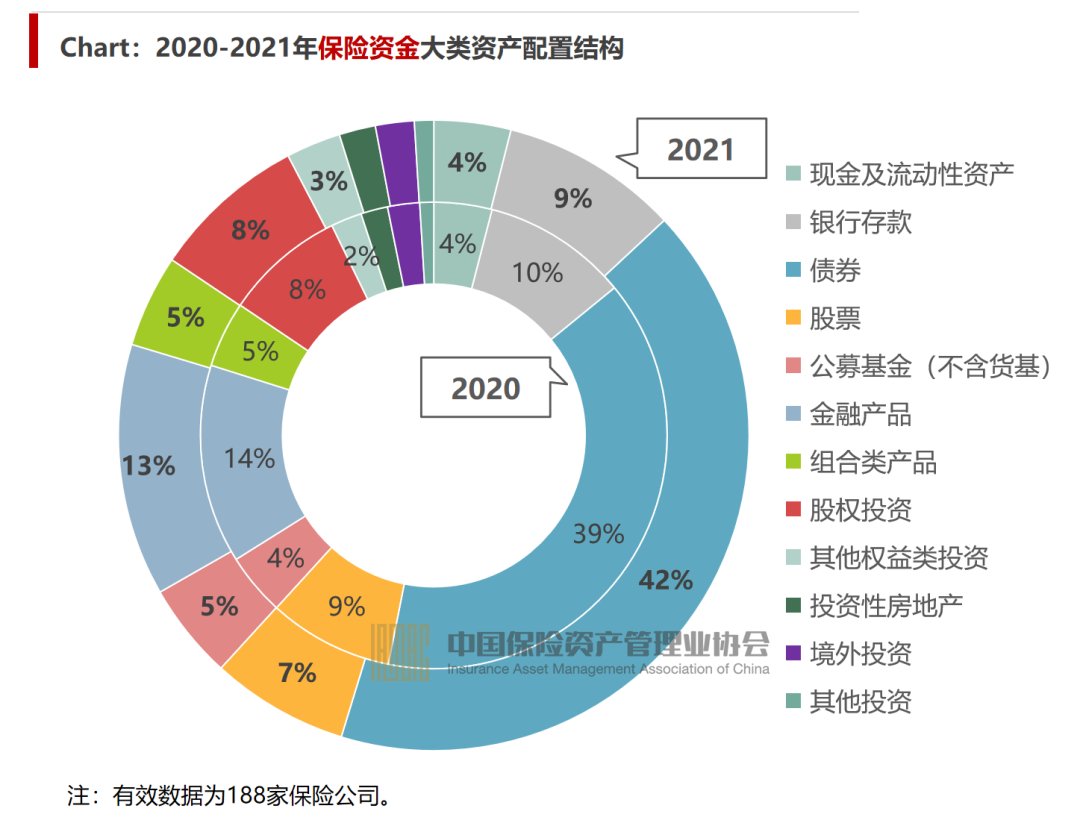
\includegraphics[width=0.6\linewidth]{img/stats.jpeg}
            \caption{保险资金运用的形式}
        \end{figure}
    }
\end{frame}

\begin{frame}
    \frametitle{运用范围:存款及有价证券}
    随着时代发展,后来运用范围加入了科创板、北交所、REITs等新投资品种。并且比例监管方面也有所放松,上季度综合偿付能力充足率为350\%以上的,权益类资产投资余额最高可占上季末总资产的45\%。
    \begin{enumerate}
        \item 禁止存款于非银行金融机构,且投资资产不能用于提供担保或贷款(保单质押贷款除外)
        \item 债券应达到原保监会认可的信用评级机构评定的、且符合规定要求的信用级别。\textbf{可以投资资产证券化产品}
        \item 保险资金开展股票投资,分为一般股票投资、重大股票投资和上市公司收购等,原保监会根据不同情形实施差别监管。不得买入ST、*ST股票。
        \item 基金限制反而有所放松,不再要求“净资产连续三年保持在人民币一亿元以上”。
    \end{enumerate}
\end{frame}
\begin{frame}
    \frametitle{运用范围:不动产}
    \begin{block}{第十三条}
        保险集团(控股)公司、保险公司购置自用不动产……应当使用自有资金(此前为“不得使用各项准备金”)。
    \end{block}
    \only<1>{
        保险公司不得\textbf{直接}从事房地产开发建设,也不能投资不符合国家产业政策的企业股权和不动产,但是可以设立不动产、基础设施、养老等专业保险资产管理机构。
    }
    \only<2>{
        \begin{figure}[H]
            \centering
            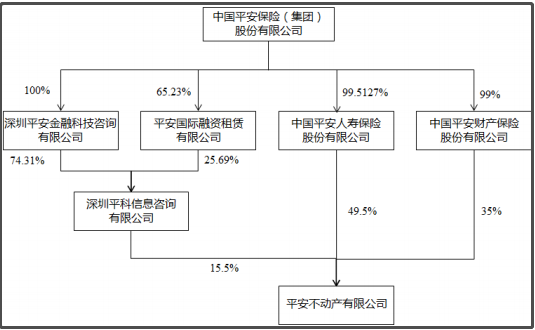
\includegraphics[width=0.6\linewidth]{img/pingan.png}
        \end{figure}
    }
\end{frame}
\begin{frame}
    \frametitle{运用范围:股权}
    保险资金做VC的LP在2010版的办法明令禁止,但是在2017版放开。2022年截至11月,金融机构LP出资272起,险资排名第一,其出资次数占比为30\%
    \begin{itemize}
        \item 举牌上市公司或者从事对其他企业实现控股的股权投资应当使用自有资金
        \item 实现控股的股权投资应当限于保险类企业、非保险类金融企业、与保险业务相关的企业
        \item 保险资金可以投资创业投资基金等私募基金
        \item 保险资金可以投资设立不动产、基础设施、养老等专业保险资产管理机构,专业保险资产管理机构可以设立符合条件的保险私募基金
        \item 保险集团(控股)公司、保险公司的重大股权投资,应当报保监会核准
    \end{itemize}
\end{frame}

\begin{frame}
    \frametitle{资金运用模式:自主投资或委托投资}
    \begin{itemize}
        \item \textbf{要求}:“集中管理、统一配置、专业运作”,实行保险资金的集约化、专业化管理。
        \item \textbf{投资管理}:保险资金应当由法人机构统一管理和运用,分支机构不得从事保险资金运用业务。
        \item \textbf{资金托管}:托管的保险资产独立于托管机构固有资产和托管的其他资产(托管机构破产也不影响)
        \item \textbf{资产登记}:18版新提出
        \item \textbf{如果委托投资}:确保委托人、受托人、托管人职责独立,受托人需要将不同委托机构资金独立管理
    \end{itemize}

\end{frame}
\begin{frame}
    \frametitle{资金运用模式:委托投资}
    委托人:保险公司,不得要求最低投资收益保证、非法转移保险利润,要求受托人提供其他委托机构信息

    受托人:专业投资管理机构,不得混合管理自有、受托资金或者不同委托机构资金,不得挪用或通道业务

    托管人:通常是银行
    \begin{figure}[H]
        \centering
        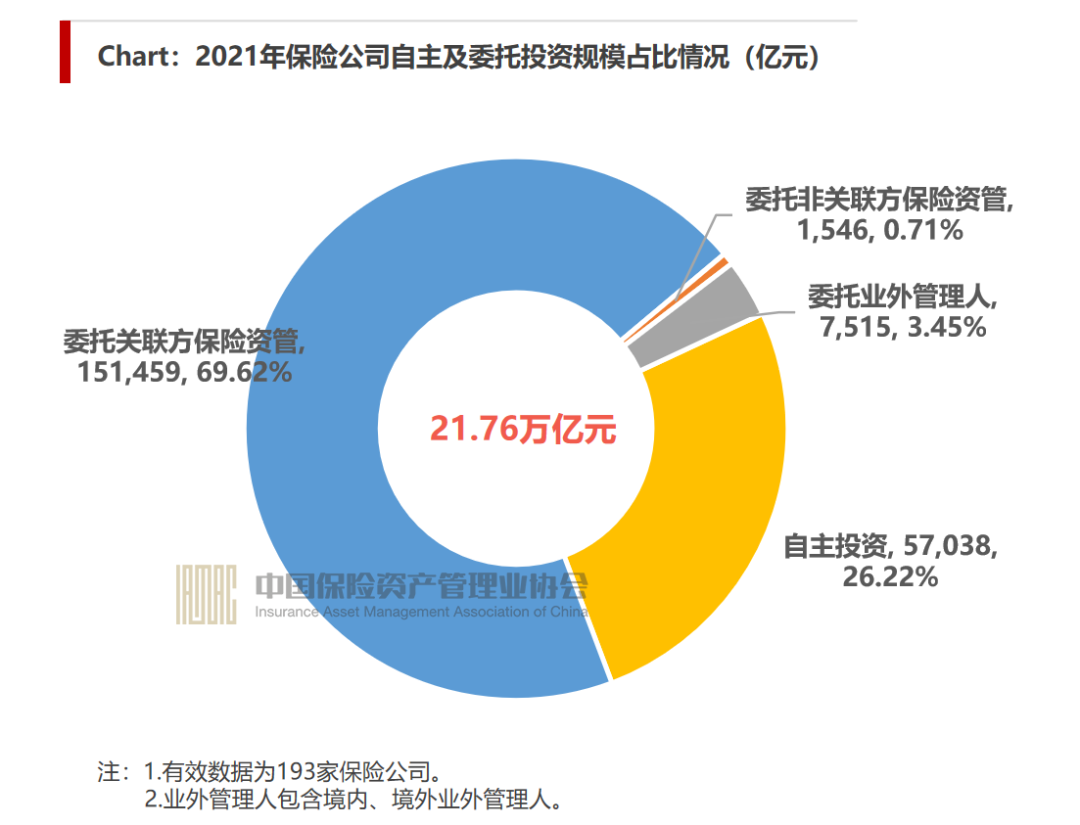
\includegraphics[width=0.6\linewidth]{img/trust.jpeg}
    \end{figure}
\end{frame}
\begin{frame}
    \frametitle{资金运用模式:限制通道和嵌套}

    金融去杠杆、资管新规逐步落实的背景下,《管理办法》禁止:
    \begin{itemize}
        \item 投资管理人将受托资金转委托
        \item 为委托机构提供通道服务
        \item 受托人提供最低投资收益保证。
    \end{itemize}
    \begin{figure}[H]
        \centering
        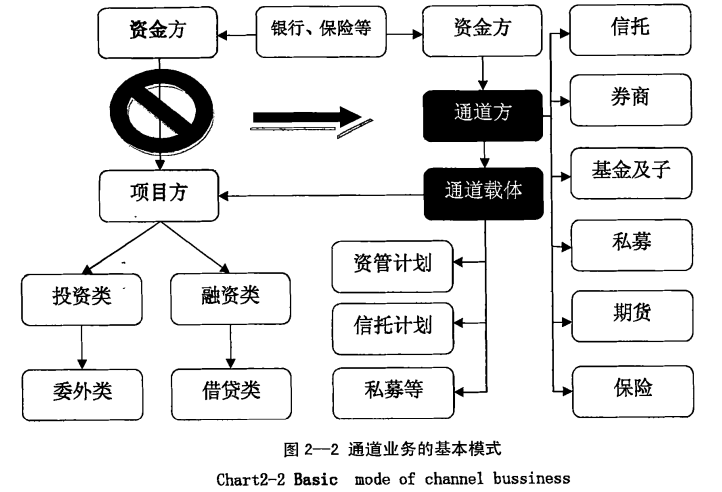
\includegraphics[width=0.6\linewidth]{img/channel.png}
    \end{figure}

\end{frame}
\subsection{决策运行机制}
\begin{frame}
    \frametitle{组织结构与职责}
    \begin{itemize}
        \item \textbf{董事会负责制}。董事会对资产配置和投资政策、风险控制、合规管理承担最终责任,董事会应当设立具有投资决策、资产负债管理和风险管理等相应职能的专业委员会。重大保险资金运用事项,应当经董事会审议通过。
        \item 管理层根据董事会授权负责保险资金运用的日常运营和管理
        \item \textbf{保险公司设置专门的保险资产管理部门},独立于财务、精算、风控等其他业务部门。除一般资管机构要求外,自行投资时,资管部门负责日常投资和交易;委托投资时,资管部门监督投资行为和评估投资业绩等。
        \item \textbf{保险资管机构应当设立首席风险管理执行官},独立向董事会、中国保监会报告有关情况,且不得主管投资业务。
    \end{itemize}
\end{frame}
\begin{frame}
    \frametitle{资金运用流程}
    \begin{itemize}
        \item 保险集团(控股)公司、保险公司管理制度和内部控制机制:
              \begin{itemize}
                  \item 资产配置相关制度
                  \item 投资研究、决策和授权制度
                  \item 交易和结算管理制度
                  \item 绩效评估和考核制度
                  \item 信息系统管理制度
                  \item 风险管理制度等
              \end{itemize}
        \item 保险资金配置:以独立法人为单位,统筹境内境外两个市场
        \item 建立专业化分析平台和投资决策和授权制度,建立和完善公平交易机制(风险隔离、集中度管理等)
        \item 以资产负债管理为核心的绩效评估体系,推进长期投资、价值投资和分散化投资
        \item 建立保险资金运用信息管理系统
    \end{itemize}
\end{frame}
\subsection{风险管控与监督管理}
\begin{frame}
    \frametitle{风险管控}
    \begin{itemize}
        \item \textbf{目标}:建立全面覆盖、全程监控、全员参与的保险资金运用风险管理组织体系和运行机制,管理和控制资产负债错配风险、流动性风险、市场风险、信用风险等
        \item \textbf{不可为}:严格控制融资规模和杠杆,禁止投机或者用短期拆借资金投资高风险和流动性差的资产,参与衍生产品交易仅限于对冲风险,不得用于投机
        \item \textbf{可为}:
              \begin{itemize}
                  \item \textbf{建立风险责任人制度},明确相应的风险责任人;
                  \item 建立内部稽核和外部审计制度,每年至少一次
                  \item 建立保险资金运用风险处置机制
                  \item 确保风控人员具有履行职责所需知情权和查询权
              \end{itemize}
    \end{itemize}
\end{frame}
\begin{frame}
    \frametitle{监督管理}
    \begin{itemize}
        \item \textbf{监管方式}:原保监会采用现场监管与非现场监管相结合的方式,对保险集团(控股)公司、保险公司保险资金运用实行分类监管、持续监管、风险监测和动态评估
        \item \textbf{投资前}:分管投资的高管等需在任职前取得原保监会核准的任职资格;首席投资官由分管投资的高级管理人员担任,有任命和报告的义务;重大股权投资应报保监会核准;保险资产管理产品,实行核准、备案或注册管理。
        \item \textbf{投资中}:保监会有权要求保险公司提供报告、报表、文件和资料;重大投资决议在5个工作日内向保监会报告。
        \item \textbf{违规处罚}:原保监会可以限制其资金运用的形式和比例;可以责令限期改正、进行监管谈话;给予行政处罚(对保险公司:罚款、限制业务范围、责令停止接受新业务或者吊销业务许可证;对相关人员:警告、罚款、撤销任职资格、禁止进入保险业)等。
    \end{itemize}
\end{frame}
\section{关于加强和改进保险资金运用比例监管的通知(2014)}
\begin{frame}
    \frametitle{资金与资产}
    \begin{figure}
        \begin{minipage}{.48\textwidth}
            \centering
            
\includegraphics[width=\linewidth]{img/money.jpeg}
            \caption{资金}
        \end{minipage}
        \begin{minipage}{.48\textwidth}
            \centering
            
\includegraphics[width=\linewidth]{img/asset.jpeg}
            \caption{资产}
        \end{minipage}
    \end{figure}
    通知所称的总资产应当扣除债券回购融入资金余额和独立账户资产金额,独立账户资产包括投连险、变额年金、健康/养老保障委托管理产品和非寿险非预定收益投资型保险产品等资产
\end{frame}
\subsection{保险资产分类及定义}
\begin{frame}
    \frametitle{保监会定义下的资产分类}
    保险公司投资资产划分为流动性资产、固定收益类资产、权益类资产、不动产类资产和其他金融资产等五大类资产。保险公司应当\textbf{合并计算}投资境内和境外的大类资产监管比例。
    \begin{enumerate}
        \item<1-> \textbf{流动性资产}\only<1>{
                。主要包括现金、货币市场基金、银行活期存款、银行通知存款、1 年内到期政府债券等,境外品种还包括1 年内到期的\textbf{商业票据、公司债券、可转换债券}。
                \begin{figure}[H]
                    \centering
                    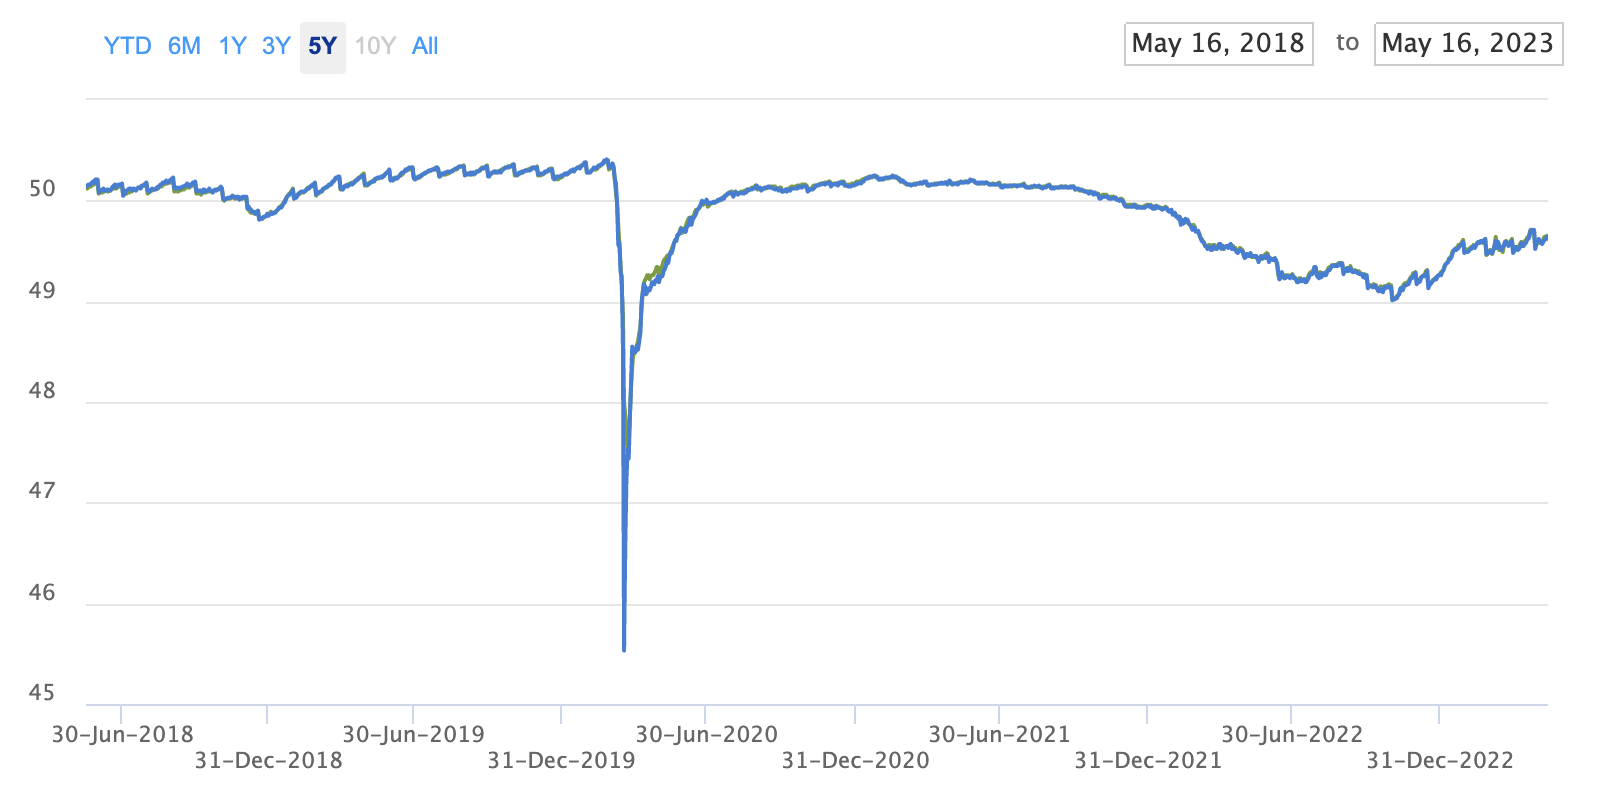
\includegraphics[width=0.6\linewidth]{img/bond.png}
                    \caption{久期0.45年的美国公司债ETF走势}
                \end{figure}
            }
        \item<2-> \textbf{固定收益类资产}\only<2>{
                。包括银行定期存款、银行协议存款、债券型基金、固收类保险资产管理产品、金融债、企业债、公司债和剩余期限在1年以上的政府债券
            }
        \item<3-> \textbf{权益类资产}\only<3>{
                。包括上市权益类资产和未上市权益类资产。其中境内上市权益类资产最初仅包括沪深主板,后续逐渐开放。
            }
        \item<4> \textbf{不动产类资产}\only<4>{
                。境内包括不动产、基础设施投资计划及其他不动产相关金融产品等,境外品种主要包括商业不动产、办公不动产和REITs等。后续国内REITs也纳入不动产类资产。
            }

        \item<2-> \textbf{其他金融资产}\only<2>{
                。包括银行理财、ABS、集合资金信托计划、专项资管计划、其他保险资产管理产品
            }
    \end{enumerate}
\end{frame}

\subsection{大类资产监管比例}
\begin{frame}
    \frametitle{最初的比例限制}
    为防范系统性风险,针对保险公司配置大类资产制定保险资金运用上限比例。
    \begin{table}
        \centering
        \begin{tabular}{lll}
            \begin{tabular}{lll}
                \toprule
                大类资产账面余额                             & 占   & 上限比例  \\ \midrule
                权益类\footnote{不包括保险公司以自有资金投资的保险类企业股权} & 总资产 & 30\%  \\
                \qquad 重大股权投资                        & 净资产 & 100\% \\
                不动产类\footnote{不包括保险公司购置的自用性不动产}      & 总资产 & 30\%  \\
                \qquad 自用性不动产                        & 净资产 & 50\%  \\
                其他金融资产                               & 总资产 & 25\%  \\
                境外投资                                 & 总资产 & 15\%  \\ \bottomrule
            \end{tabular}
        \end{tabular}
    \end{table}
\end{frame}
\begin{frame}
    \frametitle{比例限制的调整}
    \begin{enumerate}
        \item 2015年股灾期间,原保监会《关于提高保险资金投资蓝筹股票监管比例有关事项的通知》“投资权益类资产的余额占上季度末总资产比例达到30\%的,可进一步增持蓝筹股票,增持后权益类资产余额不高于上季度末总资产的40\%”。
        \item 2017年经历举牌风波后,监管部门将权益类资产占保险公司总资产比例从40\%下调至30\%,恢复至2014年的通知要求。
        \item 2020年原银保监会《关于优化保险公司权益类资产配置监管有关事项的通知》实施差异化的审慎监管,根据综合偿付能力充足率不同,将权益类资产占比上限分别设置为10\% - 45\%。
        \item 事实上整体险资权益配置始终低于15\%
    \end{enumerate}
\end{frame}

\subsection{集中度风险监管比例}
\begin{frame}
    \frametitle{集中度风险监管比例}
    \begin{enumerate}
        \item 投资单一固收类资产、权益类资产、不动产类资产、其他金融资产的账面余额,均不高于本公司上季末总资产的5\%\footnote{15年股灾期间上浮投资单一蓝筹股的比例上限为10\%}。
        \item 【条款废止】\footnote{2017年《关于进一步加强保险资金股票投资监管有关事项的通知》废止}投资上市公司股票,有权参与上市公司的财务和经营政策决策,或能够对上市公司实施控制的,纳入股权投资管理,遵循保险资金投资股权的有关规定(长期股权投资按照成本法或权益法核算,而非按公允价值计量,避免股价波动带来大幅影响)。
        \item 投资单一法人主体的余额,合计不高于本公司上季末总资产的20\%。
    \end{enumerate}
\end{frame}
\subsection{风险监测比例}
\begin{frame}
    \frametitle{风险监测比例}
    \textbf{监测比例不同于监管比例},保险公司存在以下情形的,应当于该事项发生后 5 个工作日内向原保监会报告:
    \begin{enumerate}
        \item 流动性监测:流动性资产占比低于5\%(财产险公司为7\%)
        \item 融资杠杆监测:同业拆借、债券回购等融入资金余额合计占比高于 20\%。
        \item 类别资产监测:AA及以下长信用债占比超10\%、权益类或不动产类超20\%(监管比例30\%)、其他类或境外投资超15\%(监管比例分别25\%/15\%)。
        \item 单一保险资产管理产品占比高于 5\%
    \end{enumerate}
\end{frame}
\subsection{内控比例管理}
\begin{frame}
    \frametitle{内控比例管理}
    \begin{block}{五、内控比例管理}
        \begin{itemize}
            \item 保险公司应当按照资产负债管理和资产配置要求,制定分散投资管理制度和风险控制措施,严格控制大类资产投资比例、高风险资产投资比例、行业和单一品种以及单一交易对手投资比例等。同时,还应当制定流动性风险、信用风险、市场风险等风险预警监测比例。保险公司应当密切监控相关风险敞口,确保其在自身风险承受能力和资本覆盖能力之内。
            \item 保险公司应当制定流动性风险管理方案,包括流动性风险管理体系和治理结构,管理策略和重要政策,识别、计量和监测流动性风险的主要方法和程序,流动性风险状况评价指标 压力测试和应急预案等,切实防范流动性风险。
        \end{itemize}
    \end{block}

\end{frame}
\subsection{监督管理}
\begin{frame}
    \frametitle{监督管理}
    \begin{itemize}
        \item \textbf{违反监管比例}:责令限期改正。客观原因导致的不得增加相关投资,5个工作日内向保监会报告,并限期调整投资比例。
        \item \textbf{超过监测比例}:5个工作日内向保监会报告,并披露相关信息,否则对高管进行监管谈话,列示保险公司不良记录。
        \item \textbf{内控比例}:向保监会报告,并于每年在上年度资产配置执行情况报告中,向保监会报告比例实际执行情况。
        \item \textbf{信息登记}:实际支付投资款项后5个工作日内,向信息登记平台报送投资合同及产品信息。

        \item \textbf{特别监管措施}:存在重大经营问题、重大投资风险的,增加信息披露内容、提高信息披露频率等。偿付能力状况不符合要求的,限制保险资金运用形式、比例等。未按有关规定运用保险资金的,限期改正并处以罚款;情节严重的,责令调整负责人及有关管理人员,限制其业务范围、责令停止接受新业务或者吊销业务许可证。
    \end{itemize}
\end{frame}
\end{document}
